\documentclass[border=3pt]{standalone}
% Shared preamble of the block diagrams: LaTeX fonts (Latin Modern, as in the thesis text) and TikZ styles.
% Compile with build.sh (needs pdflatex + TikZ). In the thesis, just include the compiled PDFs.
\usepackage[T1]{fontenc}
\usepackage{lmodern}
\usepackage{amsmath,amssymb,bm}
\usepackage{tikz}
\usetikzlibrary{arrows.meta,calc,fit,backgrounds}

\definecolor{boxblue}{RGB}{218,232,245}   \definecolor{edgeblue}{RGB}{143,180,220}
\definecolor{boxgreen}{RGB}{226,240,217}  \definecolor{edgegreen}{RGB}{140,190,120}
\definecolor{boxteal}{RGB}{213,238,240}   \definecolor{edgeteal}{RGB}{110,190,196}
\definecolor{boxpurple}{RGB}{232,224,243} \definecolor{edgepurple}{RGB}{170,140,205}
\definecolor{boxorange}{RGB}{252,228,214} \definecolor{edgeorange}{RGB}{240,160,115}
\definecolor{fwdc}{RGB}{62,106,153}       \definecolor{invc}{RGB}{232,98,44}
\definecolor{navy}{RGB}{31,58,95}         \definecolor{muted}{RGB}{90,100,115}

\tikzset{
  >=Stealth,
  icon/.style  ={draw=edgeblue, fill=boxblue, rounded corners=3pt, line width=0.6pt, minimum width=1.5cm, minimum height=1.15cm},
  block/.style ={draw=edgeblue, fill=boxblue, rounded corners=3pt, line width=0.6pt, align=center, text=navy, inner sep=4pt, font=\small},
  plain/.style ={draw=black, fill=white, rounded corners=3pt, line width=0.8pt, align=center, inner sep=4pt, font=\small},
  fwd/.style   ={-{Stealth[length=5pt,width=4pt]}, line width=0.9pt, color=fwdc},
  inv/.style   ={-{Stealth[length=5pt,width=4pt]}, line width=0.9pt, color=invc, dash pattern=on 3pt off 2pt},
  group/.style ={rounded corners=4pt, line width=0.9pt, dash pattern=on 4pt off 3pt},
  note/.style  ={font=\footnotesize, text=muted, align=center},
}
% plate icon: rectangle with resonator dots; #1 centre, #2 dots "x/y, x/y" in [-1,1]
\newcommand{\plateicon}[2]{\begin{scope}[shift={#1}]
  \draw[line width=0.7pt] (-0.55,-0.25) rectangle (0.55,0.25);
  \foreach \px/\py in {#2} {\fill (0.5*\px,0.19*\py) circle (1.7pt);}
\end{scope}}
% sketch of an ERP spectrum; #1 centre
\newcommand{\spectrumicon}[1]{\begin{scope}[shift={#1}]
  \draw[line width=0.6pt] (-0.55,0.42)--(-0.55,-0.40)--(0.55,-0.40);
  \draw[line width=0.85pt, line join=round, line cap=round] (-0.5,-0.32) -- (-0.3,-0.12) -- (-0.22,0.02) -- (-0.17,0.30) -- (-0.11,-0.02)
     -- (-0.02,0.14) -- (0.04,-0.08) -- (0.12,-0.02) -- (0.18,0.24) -- (0.24,-0.12) -- (0.38,0.0) -- (0.50,0.10);
\end{scope}}

\begin{document}
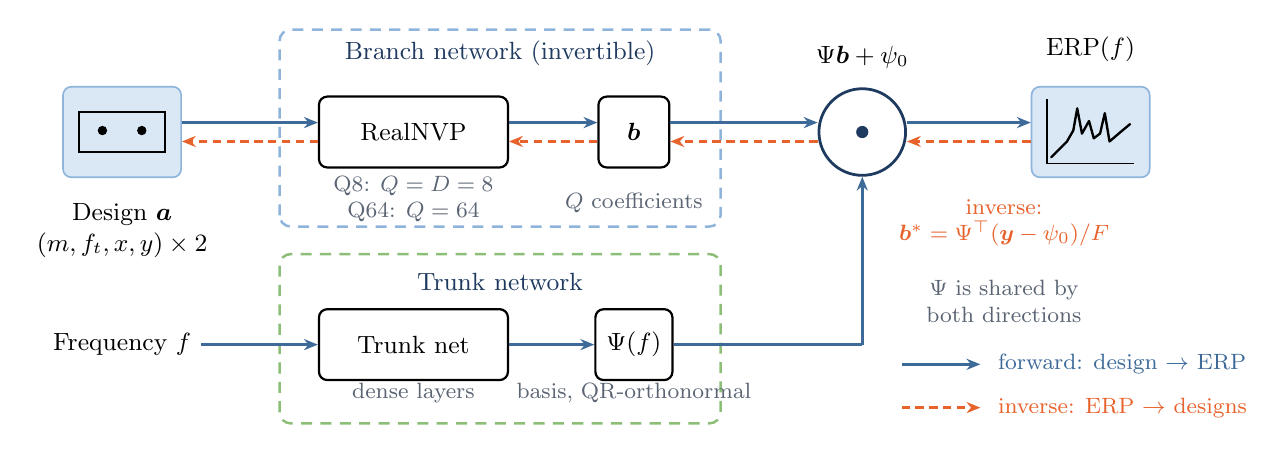
\begin{tikzpicture}
% design and frequency inputs
\node[icon] (des) at (0,1.7) {}; \plateicon{(des.center)}{-0.5/0.1, 0.5/0.1}
\node[font=\small, align=center] at (0,0.45) {Design $\bm a$\\ $(m,f_t,x,y)\times 2$};
\node[font=\small] (freq) at (0,-1.0) {Frequency $f$};
% branch network (invertible)
\draw[group, draw=edgeblue] (2.0,0.5) rectangle (7.6,3.0);
\node[font=\small, text=navy] at (4.8,2.7) {Branch network (invertible)};
\node[plain, minimum width=2.4cm, minimum height=0.9cm] (nvp) at (3.7,1.7) {RealNVP};
\node[plain, minimum width=0.9cm, minimum height=0.9cm] (b) at (6.5,1.7) {$\bm b$};
\node[note] at (3.7,0.85) {Q8: $Q=D=8$\\ Q64: $Q=64$};
\node[note] at (6.5,0.8) {$Q$ coefficients};
% trunk network
\draw[group, draw=edgegreen] (2.0,-2.0) rectangle (7.6,0.15);
\node[font=\small, text=navy] at (4.8,-0.2) {Trunk network};
\node[plain, minimum width=2.4cm, minimum height=0.9cm] (trunk) at (3.7,-1.0) {Trunk net};
\node[note] at (3.7,-1.62) {dense layers};
\node[plain, minimum width=0.9cm, minimum height=0.9cm] (psi) at (6.5,-1.0) {$\Psi(f)$};
\node[note] at (6.5,-1.62) {basis, QR-orthonormal};
% combination and output
\node[circle, draw=navy, line width=1.0pt, minimum size=1.1cm, inner sep=0] (sum) at (9.4,1.7) {};
\fill[navy] (sum.center) circle (2.2pt);
\node[font=\small] at (9.4,2.65) {$\Psi\bm b+\psi_0$};
\node[icon] (out) at (12.3,1.7) {}; \spectrumicon{(out.center)}
\node[font=\small] at (12.3,2.75) {ERP$(f)$};
% forward path
\draw[fwd] ($(des.east)+(0,0.12)$) -- ($(nvp.west)+(0,0.12)$);
\draw[fwd] ($(nvp.east)+(0,0.12)$) -- ($(b.west)+(0,0.12)$);
\draw[fwd] ($(b.east)+(0,0.12)$) -- ($(sum.west)+(0,0.12)$);
\draw[fwd] ($(sum.east)+(0,0.12)$) -- ($(out.west)+(0,0.12)$);
\draw[fwd] (freq.east) -- (trunk.west);  \draw[fwd] (trunk.east) -- (psi.west);
\draw[fwdc, line width=0.9pt] (psi.east) -- (9.4,-1.0);  \draw[fwd] (9.4,-1.0) -- (sum.south);
% inverse path
\draw[inv] ($(out.west)+(0,-0.12)$) -- ($(sum.east)+(0,-0.12)$);
\draw[inv] ($(sum.west)+(0,-0.12)$) -- ($(b.east)+(0,-0.12)$);
\draw[inv] ($(b.west)+(0,-0.12)$) -- ($(nvp.east)+(0,-0.12)$);
\draw[inv] ($(nvp.west)+(0,-0.12)$) -- ($(des.east)+(0,-0.12)$);
\node[font=\footnotesize, text=invc, align=center] at (11.2,0.55) {inverse:\\ $\bm b^{\ast}=\Psi^{\top}(\bm y-\psi_0)/F$};
\node[note] at (11.2,-0.45) {$\Psi$ is shared by\\ both directions};
% legend
\draw[fwd] (9.9,-1.25) -- (10.9,-1.25); \node[note, anchor=west, text=fwdc] at (11.0,-1.25) {forward: design $\to$ ERP};
\draw[inv] (9.9,-1.8) -- (10.9,-1.8);   \node[note, anchor=west, text=invc] at (11.0,-1.8) {inverse: ERP $\to$ designs};
\end{tikzpicture}
\end{document}
